\documentclass[aspectratio=169]{beamer}
\usetheme{metropolis}
\usecolortheme{default}

\usepackage{coffee4}
\usepackage{color}
\usepackage{graphicx}
\usepackage{amssymb}
\usepackage{amsmath}
\usepackage{wasysym}
\usepackage{tabularx, booktabs}
\usepackage[lined]{algorithm2e}

% For text bubble
\usepackage{tikz}
\usetikzlibrary{shapes,fit,backgrounds}
\newcounter{mybox}
\newcommand\tikzmark[1]{%
  \tikz[remember picture,overlay] \node[inner xsep=0pt] (#1) {};
}
\newcommand<>\ColorBox[2][]{%
\stepcounter{mybox}%
\node[rectangle callout,rounded corners=5pt,draw=cyan,fill=cyan!20,align=left,#1] (box\themybox) {#2};
}

% metropolis beamer theme can be found in GitHub:
% https://github.com/matze/mtheme
% coffee stain package can be found at:
% http://hanno-rein.de/archives/349

\title{Improved Neural Relation Detection for\\ Knowledge Base Question Answering}
\author{Caleb Bryant\inst{1} Jixin Feng\inst{2}}
\institute{
Department of \\
  \inst{1}%
  Computer \& Information Science \& Engineering \\
  \inst{2}
  Electrical \& Computer Engineering\\
  University of Florida, Gainesville, FL}
\date{April 06 2018}

\begin{document}
\frame{\titlepage}

\begin{frame}
\frametitle{Paper Outline}
    \center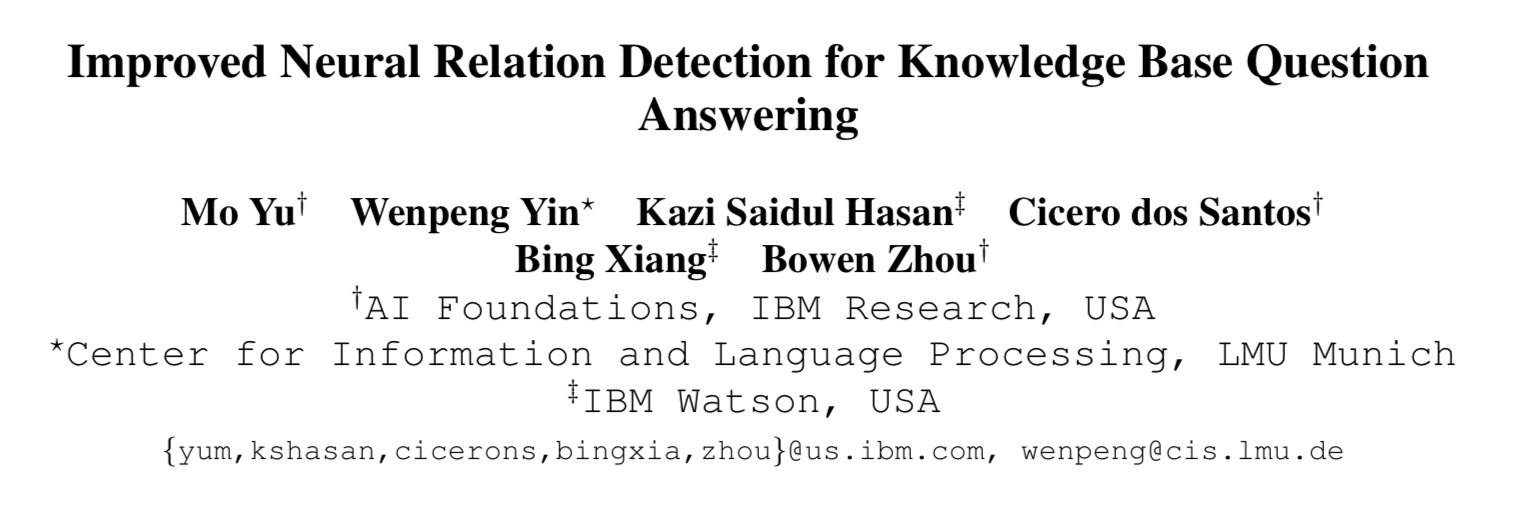
\includegraphics[width=0.7\textwidth]{figure/paper_title}
    \begin{itemize}
        \item Introduction
        \item Relation Extraction \& Relation Detection
        \item Different Granularity in KB Relations
        \item Proposed Improved Relation Detection
        \item KBQA Enhanced by Relation Detection
        \item Experiment \& Conclusion
    \end{itemize}
\end{frame}

\begin{frame}
\frametitle{What is Knowledge Base?}
    \begin{columns}
    \begin{column}{0.55\textwidth}
    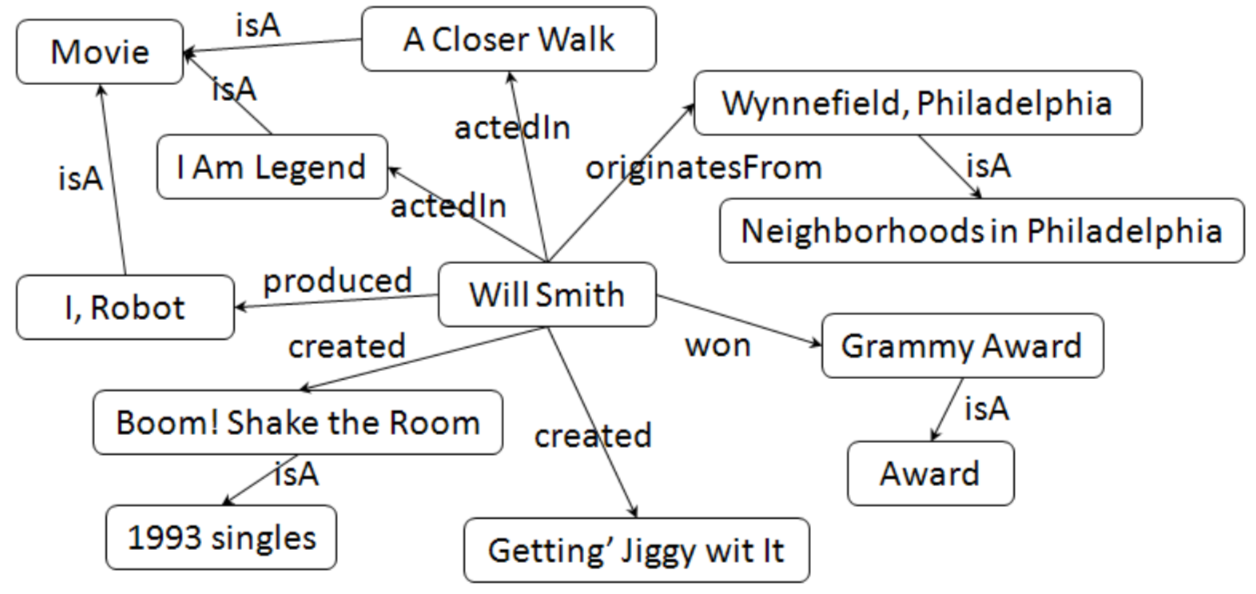
\includegraphics[width=\textwidth]{figure/KB_WS}
    % Picture Credit:
    % https://www.researchgate.net/publication/228457497_Query-Independent_Learning_to_Rank_for_RDF_Entity_Search
    \end{column}
    \begin{column}{0.45\textwidth}
    A knowledge base (KB) is a technology used to store complex 
    {\bf structured} and {\bf unstructured} information used by a computer 
    system. \\\hspace*{\fill}--{\it Wikipedia}\\
    
    It stores and manages the knowledge tuples:
    \texttt{<entity-relation-entity>}
    
    A knowledge base can be represented as graph 
    $\mathcal{G}(\mathcal{V},\mathcal{E})$, 
    if we treat entities as vertices and relations as edges.
    \end{column}
    \end{columns}
\end{frame}

\begin{frame}
\frametitle{What is a Question Answering System?}
    \begin{columns}
    \begin{column}{0.5\textwidth}
    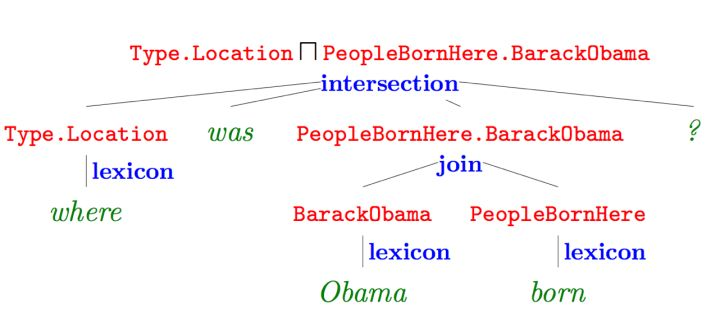
\includegraphics[width=\textwidth]{figure/KB_BO}
    % Picture Credit:
    % https://www.semanticscholar.org/paper/Semantic-Parsing-on-Freebase-from-Question-Answer-Berant-Chou/042db0977555fcd7d5eac67b26695cd918ecb44c
    Question answering (QA) is a computer systems that automatically answer questions posed by humans in a natural language. QA systems can pull answers from an unstructured collection of natural language documents.
    \end{column}
    \begin{column}{0.5\textwidth}
    
\includegraphics[width=\textwidth]{figure/IBM-Watson-Logo}
    % Picture Credit:
    % http://www.businessinsider.com/ibms-supercomputer-can-now-analyze-your-personality-based-on-a-writing-sample-heres-how-you-try-it-2015-7
    \end{column}
    \end{columns}
\end{frame}

\begin{frame}
\frametitle{What is a Question Answering System?}
    \begin{columns}
    \begin{column}{0.35\textwidth}
    \begin{itemize}
    \item {\bf IBM Watson} is automated QA system
    \item Defeated the two greatest Jeopardy! champions
    \item Won the match, outscoring both opponents combined
    \end{itemize}
    \end{column}
    \begin{column}{0.65\textwidth}
    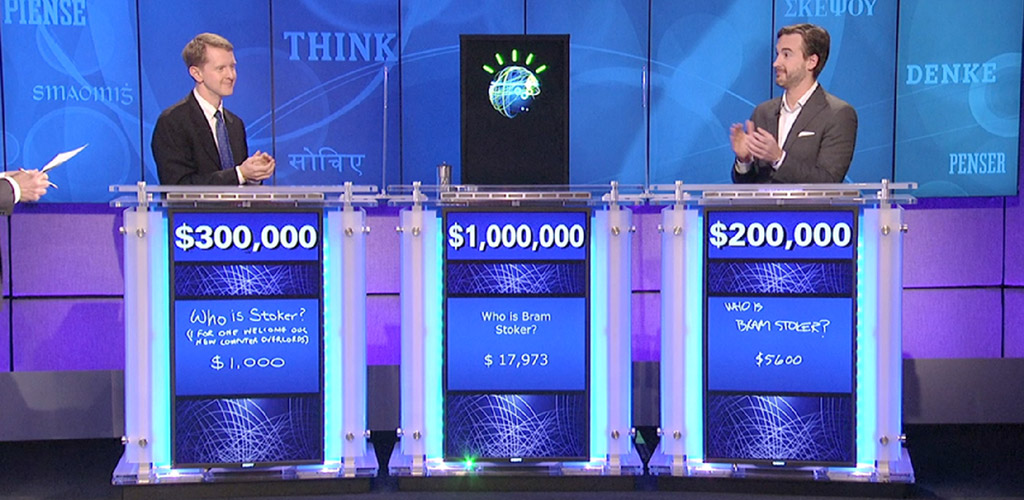
\includegraphics[width=\textwidth]{figure/Watson}
    \end{column}
    \end{columns}
\end{frame}

\begin{frame}
\frametitle{Introduction}
    \center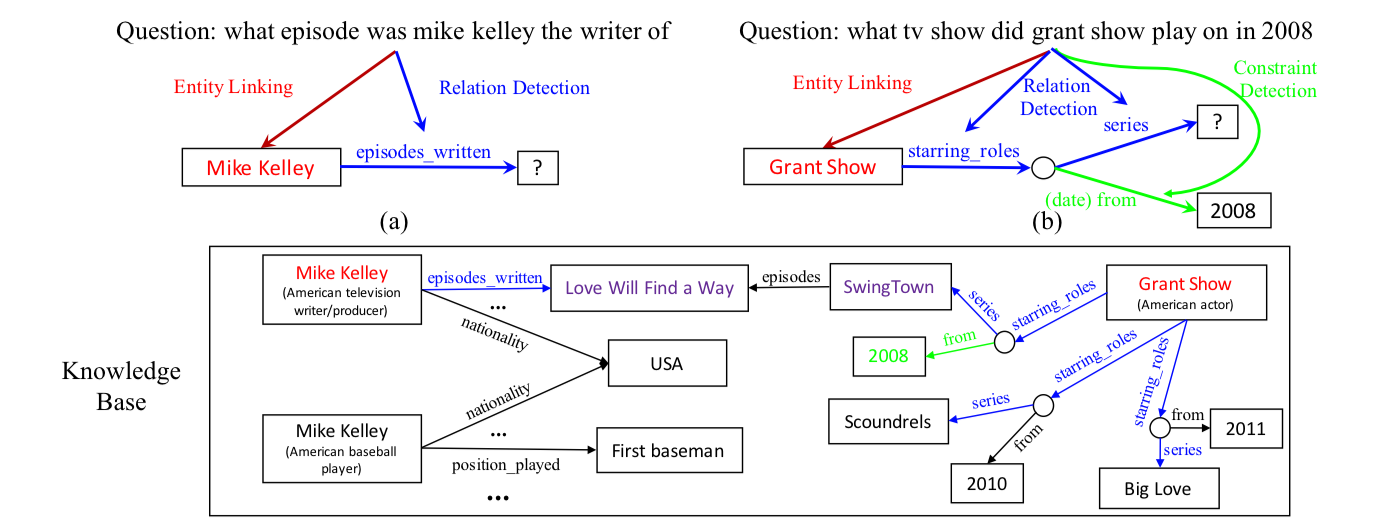
\includegraphics[width=0.8\textwidth]{figure/fig1}
    \begin{itemize}
    \item KBQA systems answer questions by obtaining information from KB tuples\\
    \item \texttt{input question} $\rightarrow$ \texttt{KB query} $\rightarrow$ \texttt{answer}
    \item Questions can be single-relation question and multiple-relation question
    \end{itemize}
\end{frame}

\begin{frame}
\frametitle{Introduction}
    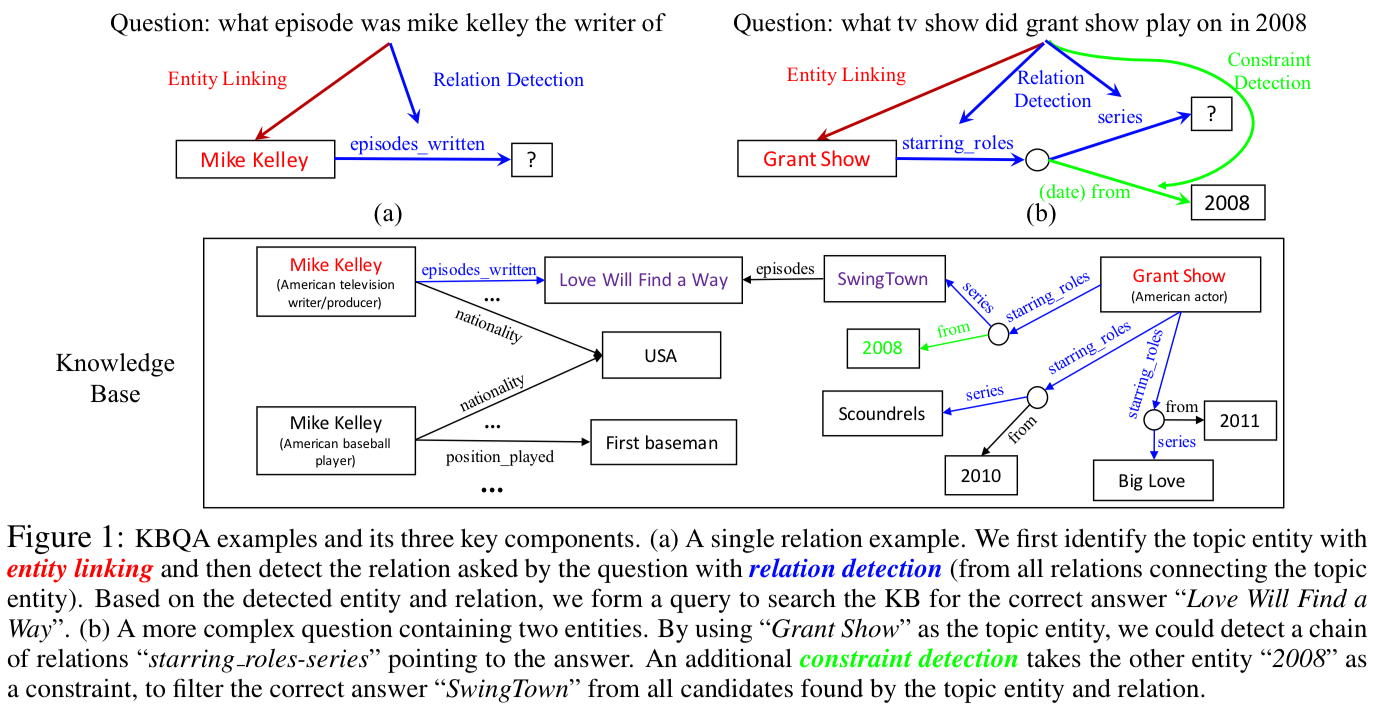
\includegraphics[width=\textwidth]{figure/fig1_big}
\end{frame}


\begin{frame}
\frametitle{Introduction}
    This paper focus on improvement of relation detection.
    \begin{itemize}
        \onslide<1->{
        \item General relation detection has been well studied in NLP
        \begin{itemize}
            \item Not KBQA driven, causing significant gap
        \end{itemize}
        \item Number of target relations is limited in most general relation detection tasks
        \begin{itemize}
            \item Normally $\leq 100$ relations detected
            \item Even a small KB may contains $\geq 6000$ relations
        \end{itemize}
        \item Multiple relation questions require a chain of prediction
        \item Relation detection in KBQA often becomes a {\bf zero-shot learning} task}
        \onslide<3->{
        \item {\bf Conclusion:} KB relation detection is much harder}
    \end{itemize}
    \onslide<2>{
    \begin{tikzpicture}[remember picture,overlay]
    \ColorBox[xshift=7cm,yshift=4.8cm]{
        Zero-shot learning is being able to solve a \\
        task despite not having received any training \\
        examples of that task. For a concrete example, \\
        imagine recognizing a category of object in \\
        photos without ever having seen a photo of \\
        that kind of object before. If you've read a \\
        very detailed description of a cat, you might \\
        be able to tell what a cat is in a photograph \\
        the first time you see it.\\
        \hspace*{\fill}--{\it Ian Goodfellow}}
        % https://www.quora.com/What-is-zero-shot-learning
    \end{tikzpicture}}
\end{frame}

\begin{frame}
\frametitle{Relation Extraction}
    \begin{itemize}
    \item The goal is to determine whether 
        \texttt{<entity-text\_paragraph-entity>} \\
        can be classified as 
        \texttt{<entity-relation-entity>}
    \item RE usually formulated as classification task
    \begin{itemize}
        \item Traditional RE relies on large amount of hand-crafted features
        \item Benefits from deep learning research: word embedding, CNN, LSTM, etc.
    \end{itemize}\pause
    \item Assume fixed, closed set of relation types to avoided zero-shot learning
    \begin{itemize}
        \item Rarely go beyond $\geq 100$ features
        \item Need to be trained in supervised way
    \end{itemize}
    \item Assume two argument entities are both available
    \begin{itemize}
        \item Question only contain single argument
    \end{itemize}
    \item Usually works on small, pre-defined relation set
    \end{itemize}
\end{frame}

\begin{frame}
\frametitle{Relation Detection}
    \begin{itemize}
        \item RD Naturally support large relation vocabulary and open relation sets
        \item Fit the goal of open-domain question answering
        \item Need to deal with zero-shot learning:
        \begin{itemize}
            \item Use pre-trained relation embeddings
            \item Factorize the relation names to sequences and use \\
            {\bf sequence matching and ranking}
        \end{itemize}
        \item Matching and ranking works well because relation names usually forms meaningful word sequences\pause
        \item This paper focus on improvement of RD
    \end{itemize}
\end{frame}

\begin{frame}
\frametitle{Different Granularity in KB Relations}
    \begin{itemize}
        \item {\bf Goal:} Formulate KB relation detection as sequence matching problem
        \item Exist different types of relation representation
        \begin{itemize}
            \item Relation Name as a Single Token ({\it relation-level})
            \item Relation as Word Sequence ({\it word-level})
        \end{itemize}
    \end{itemize}
    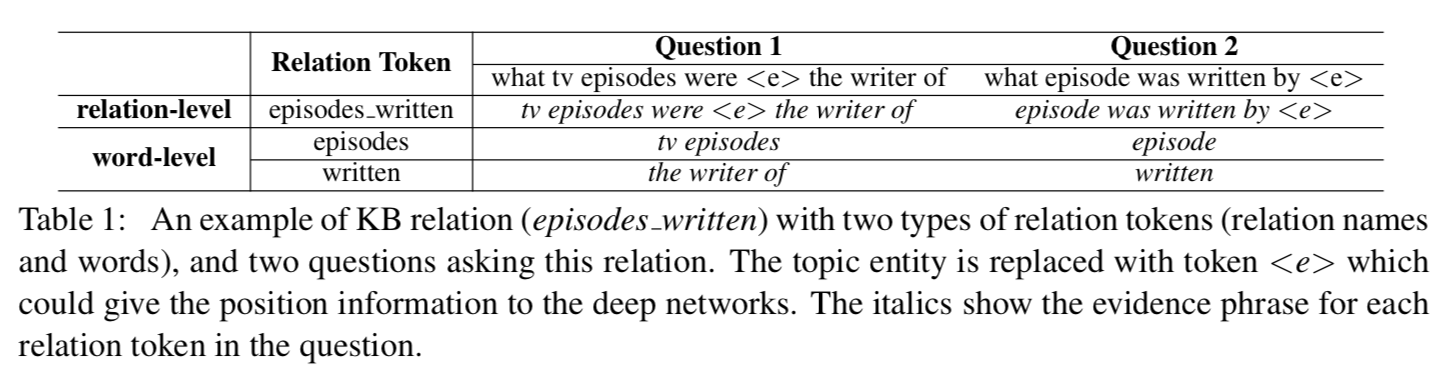
\includegraphics[width=\textwidth]{figure/table1_big}
\end{frame}

\begin{frame}
\frametitle{Relation Name as a Single Token}
    \begin{itemize}
        \item Each relation is treated as a unique token
        \item This suffers from the low relation coverage dut to limited training data
        \item In this example, matching \texttt{episodes\_written} and 
            \texttt{starring\_roles} can be hard if these names do not appear 
            in training data
        \item Relation embedding will be random vector, not comparable to question embedding
    \end{itemize}
    \center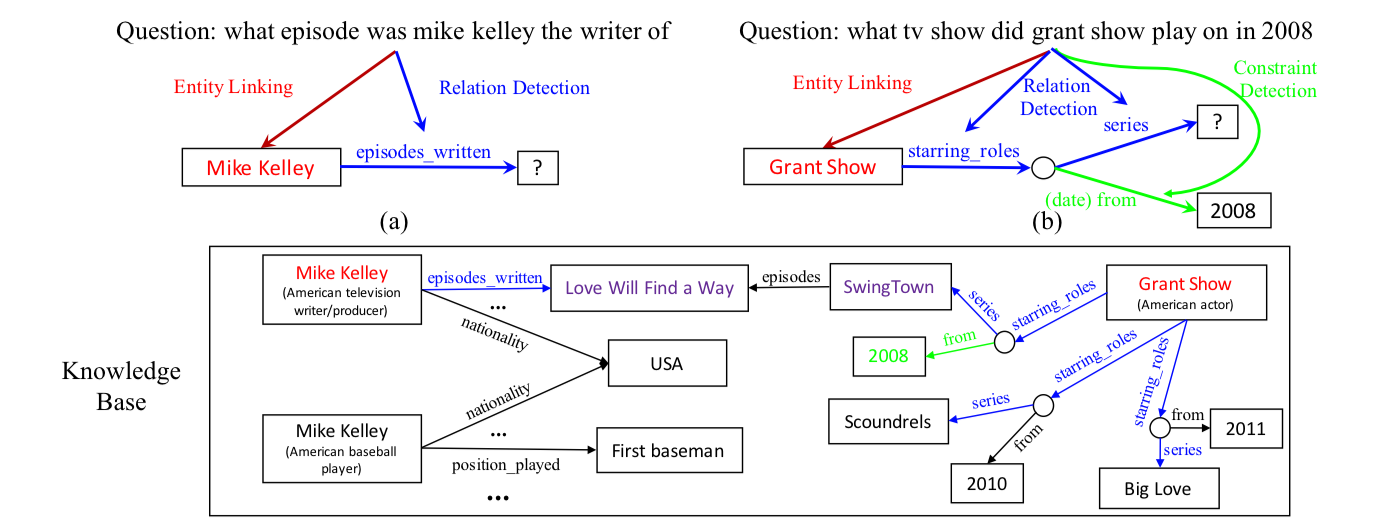
\includegraphics[width=0.8\textwidth]{figure/fig1}
\end{frame}

\begin{frame}
\frametitle{Relation as Word Sequence}
    \begin{itemize}
        \item Relation is treated as a sequence of words from the tokenized relation name
        \item Better generalization but suffers from lack of global information
        \item Very hard to rank \texttt{starring\_roles} higher than 
            \texttt{plays\_produced}
        \begin{itemize}
        \item Incorrect relation contains word ``plays''
        \item More similar to the question
        \end{itemize}
    \end{itemize}
    \center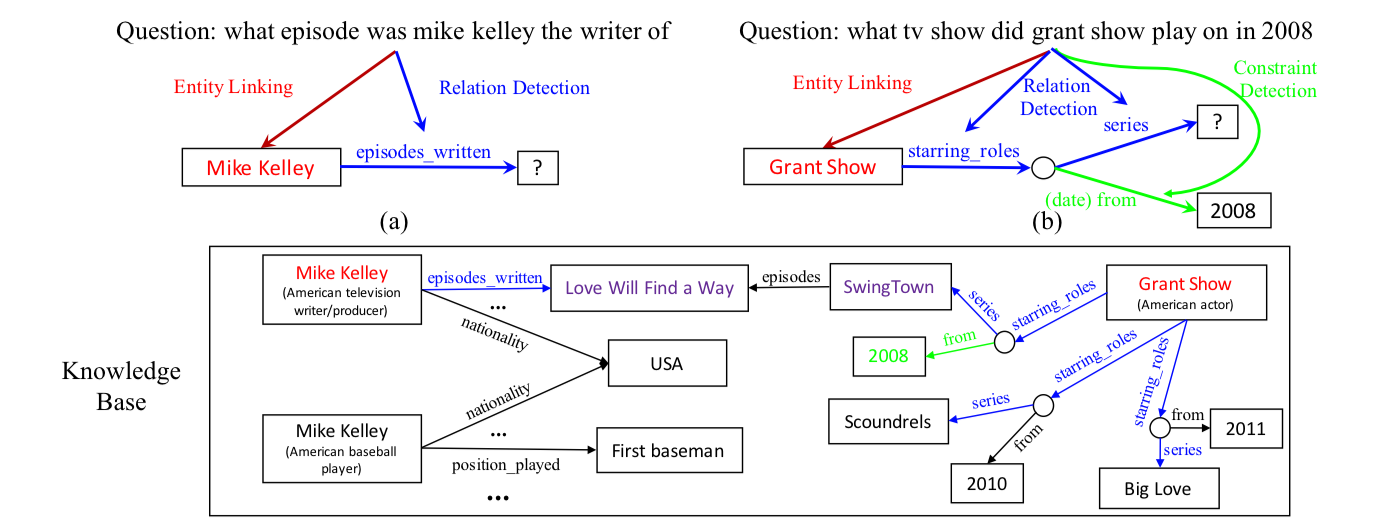
\includegraphics[width=0.8\textwidth]{figure/fig1}
\end{frame}

\begin{frame}
\frametitle{Proposed Improved Relation Detection}
    \begin{columns}
    \begin{column}{0.6\textwidth}
    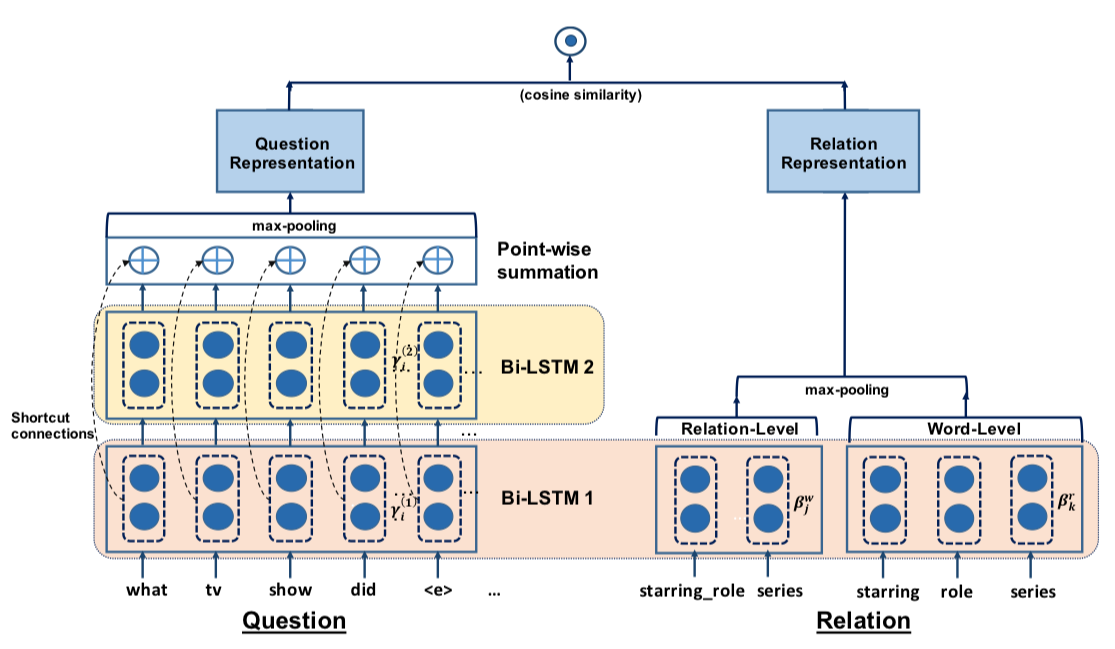
\includegraphics[width=\textwidth]{figure/sysmodel}
    \end{column}
    \begin{column}{0.4\textwidth}
    \begin{itemize}
        \item Word-level focuses more on local information but lack of global information
        \item Relation-level focus more on global information but suffer from data sparsity
        \item This paper propose a hierarchical matching approach that matches both information level
    \end{itemize}
    \end{column}
    \end{columns}
\end{frame}

\begin{frame}
\frametitle{Relation Representation from Different Granularity}
    \begin{itemize}
        \item Tokenize input relation as 
            $$\mathbf{r}=\{r_1^{word},r_2^{word},\ldots,r_{M_1}^{word}\}\cup
            \{r_1^{rel},r_2^{rel},\ldots,r_{M_2}^{rel}\}$$
        \item first $M_1$ tokens are words and last $M_2$ tokens are relation names
        \item Transform each token to word embedding then to hidden representation
            $$[\mathbf{B}_{1:M_1}^{word}:\mathbf{B}_{1:M_1}^{rel}]$$
            via two BiLSTMs
        \item Initialize relation sequence LSTMs with the final state representations of the word sequence
        \item Apply one max-pooling on these two sets of vectors and get final relation representation $\mathbf{h}^r$
    \end{itemize}
\end{frame}

\begin{frame}
\frametitle{Different Abstraction of Questions Representations}
    \begin{itemize}
        \item Want question representation vectors summarize various 
            length of phrase to match relation representations of different 
            granularity
        \item Achieved via applying deep BiLSTM on questions
        \item First layer works on word embeddings, convert question words
            $\mathbf{q}=\{q_1,\ldots,q_N\}$
            to hidden representation 
            $\mathbf{\Gamma}_{1:N}^{(1)}=[\gamma_1^{(1)},\ldots,\gamma_N^{(1)}]$
        \item Second layer convert $\mathbf{\Gamma}_{1:N}^{(1)}$ 
            to $\mathbf{\Gamma}_{1:N}^{(2)}$
        \item $\mathbf{\Gamma}_{1:N}^{(1)}$ and $\mathbf{\Gamma}_{1:N}^{(2)}$ 
            could potentially match to either level of relation representation
        \item Need additional methods to reduce difficulty
    \end{itemize}
\end{frame}

\begin{frame}
\frametitle{Hierachical Matching between Relation and Questions}
    \begin{itemize}
        \item Two levels of question hidden representation are not 
            guaranteed to be comparable
        \item Training deep BiLSTM is difficult
        \item This paper proposed two ways of Hierarchical Residual Matching
        \begin{itemize}
            \item Connecting $\gamma_i^{(1)}$ and $\gamma_i^{(1)}$, resulting
                $\gamma_i^\prime=\gamma_i^{(1)} + \gamma_i^{(2)}$, and final question
                representation $\mathbf{h}^q$ becomes a max-pooling of all $\gamma_i^\prime$
            \item Apply max-pooling on $\mathbf{\Gamma}_{1:N}^{(1)}$,
                $\mathbf{\Gamma}_{1:N}^{(2)}$ and get 
                $$\mathbf{h}^q=\mathbf{h}_{max}^{(1)}+\mathbf{h}_{max}^{(1)}$$
        \end{itemize}
        \item Matching score between relation and question is
            $$s_{rel}(\mathbf{r};\mathbf{q})=\cos(\mathbf{h}^r,\mathbf{h}^q)$$
        \item Ranking loss between golden relation $\mathbf{r}^+$ and other relations $\mathbf{r}^-$
            $$l_{rel}=\max\{0,\gamma-s_{rel}(\mathbf{r}^+;\mathbf{q})+s_{rel}(\mathbf{r}^-;\mathbf{q})\}$$
    \end{itemize}
\end{frame}

\begin{frame}
\frametitle{Hierarchical Residual BiLSTM Model}
    \center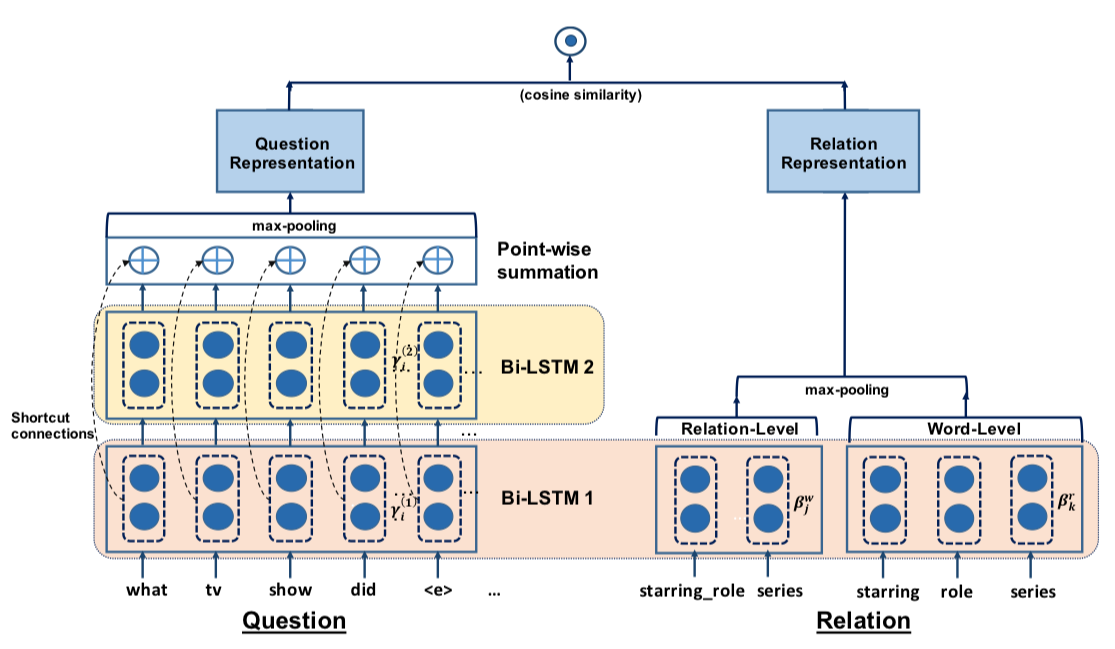
\includegraphics[width=0.8\textwidth]{figure/sysmodel}
\end{frame}

\begin{frame}
\frametitle{KBQA Enhanced by Relation Detection}
    \begin{columns}
    \begin{column}{0.48\textwidth}
    \begin{itemize}
    \item Take an existing entify linker to produce the top-K 
        linked entities $EL_K(q)$ for question $q$
    \item Generate KB queries for $q$ following a 4-step algorithm
    \end{itemize}
    \end{column}
    \begin{column}{0.52\textwidth}
    \includegraphics[width=\textwidth]{figure/algo1}
    \end{column}
    \end{columns}
\end{frame}

\begin{frame}
\frametitle{Experiment: Relation Detection}
    \onslide<1->{
    \begin{itemize}
        \item Dataset: SimpleQuestion (Bordes et al., 2015) and WebQSP (Yih et al., 2016)
        \item Each question is labeled with the gold semantic parse
        \item Direct performance evaluation is possible, as well as KBQA evaluation
    \end{itemize}}
    \onslide<2>{
    \begin{tikzpicture}[remember picture,overlay]
    \ColorBox[xshift=4cm,yshift=3cm]{Single-relation KBQA task.}
    \end{tikzpicture}}
    \onslide<3>{
    \begin{tikzpicture}[remember picture,overlay]
    \ColorBox[xshift=9cm,yshift=3cm]{Multi-relation KBQA task.}
    \end{tikzpicture}}
    \onslide<4>{
    \center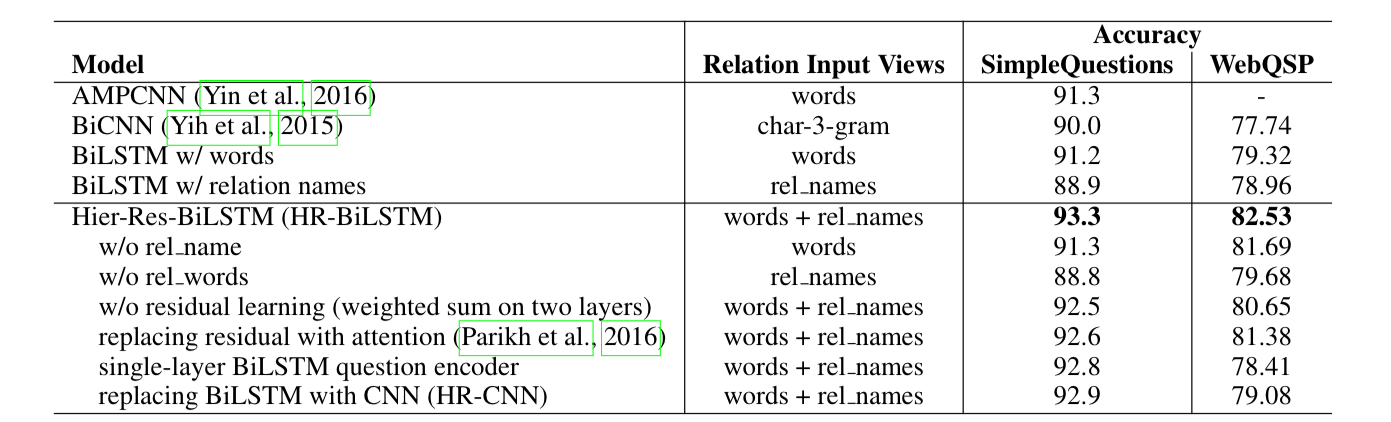
\includegraphics[width=\textwidth]{figure/table2}}
\end{frame}

\begin{frame}
\frametitle{Experiment: KBQA End-Task}
    \begin{columns}
    \begin{column}{0.5\textwidth}
    \begin{itemize}
        \item Compared to baseline relation detector, proposed system improves KBQA end-task by 2\%-3\%
    \end{itemize}
    \end{column}
    \begin{column}{0.5\textwidth}
    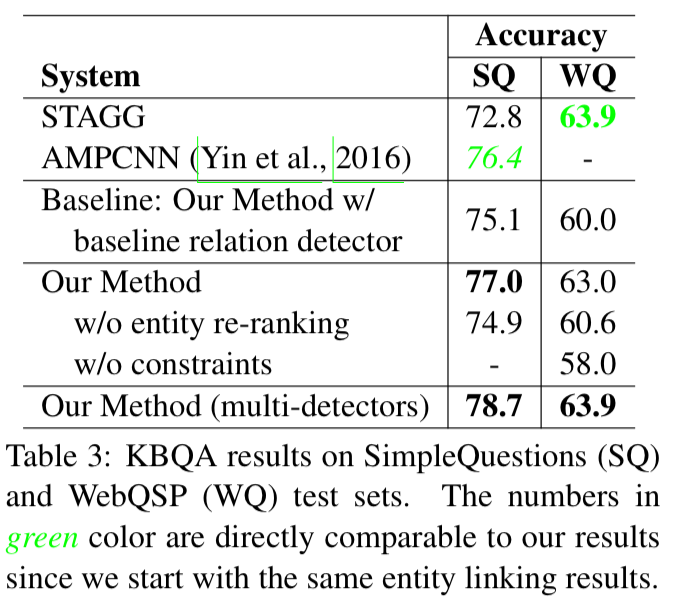
\includegraphics[width=\textwidth]{figure/table3_big}
    \end{column}
    \end{columns}
\end{frame}

\begin{frame}
\frametitle{Conclusions}
    \begin{itemize}
        \item Proposed a novel KB relation detection Model, HR-BiLSTM, that performs hierarchical matching between questions and KB relations
        \item Proposed model outperforms the previous methods on KB relation detection
        \item Proposed proof-of-concept KBQA system achieved state-of-the-arts in both single relation and multiple relation tasks
    \end{itemize}
\end{frame}

\begin{frame}
\frametitle{Conclusions}
    \begin{columns}
    \begin{column}[t]{0.5\textwidth}
    {\bf Strong Points:}
    \begin{itemize}
        \item Combine different granularity in KB relationship
            to catch both local and global information
        \item Using shortcut connections between BiLSTMs reduce training difficulty
        \item Hierarchical architecture to learn different level of abstraction to prevent over-fitting
    \end{itemize}
    \end{column}
    \begin{column}[t]{0.5\textwidth}
    {\bf Weak Points:}
    \begin{itemize}
        \item Exact analyze of training difficulty is missing
        \item Result of ablation test is not strong
        \item Overall performance improvement is marginal
    \end{itemize}
    \end{column}
    \end{columns}
\end{frame}

\begin{frame}
\Huge{Thank You!}\\
\small{Questions?}\\
\cofeAm{0.4}{0.8}{0}{120}{-10}
\end{frame}

\end{document}
